% Options for packages loaded elsewhere
\PassOptionsToPackage{unicode}{hyperref}
\PassOptionsToPackage{hyphens}{url}
%
\documentclass[
]{article}
\usepackage{amsmath,amssymb}
\usepackage{iftex}
\ifPDFTeX
  \usepackage[T1]{fontenc}
  \usepackage[utf8]{inputenc}
  \usepackage{textcomp} % provide euro and other symbols
\else % if luatex or xetex
  \usepackage{unicode-math} % this also loads fontspec
  \defaultfontfeatures{Scale=MatchLowercase}
  \defaultfontfeatures[\rmfamily]{Ligatures=TeX,Scale=1}
\fi
\usepackage{lmodern}
\ifPDFTeX\else
  % xetex/luatex font selection
\fi
% Use upquote if available, for straight quotes in verbatim environments
\IfFileExists{upquote.sty}{\usepackage{upquote}}{}
\IfFileExists{microtype.sty}{% use microtype if available
  \usepackage[]{microtype}
  \UseMicrotypeSet[protrusion]{basicmath} % disable protrusion for tt fonts
}{}
\makeatletter
\@ifundefined{KOMAClassName}{% if non-KOMA class
  \IfFileExists{parskip.sty}{%
    \usepackage{parskip}
  }{% else
    \setlength{\parindent}{0pt}
    \setlength{\parskip}{6pt plus 2pt minus 1pt}}
}{% if KOMA class
  \KOMAoptions{parskip=half}}
\makeatother
\usepackage{xcolor}
\usepackage{color}
\usepackage{fancyvrb}
\newcommand{\VerbBar}{|}
\newcommand{\VERB}{\Verb[commandchars=\\\{\}]}
\DefineVerbatimEnvironment{Highlighting}{Verbatim}{commandchars=\\\{\}}
% Add ',fontsize=\small' for more characters per line
\newenvironment{Shaded}{}{}
\newcommand{\AlertTok}[1]{\textcolor[rgb]{1.00,0.00,0.00}{\textbf{#1}}}
\newcommand{\AnnotationTok}[1]{\textcolor[rgb]{0.38,0.63,0.69}{\textbf{\textit{#1}}}}
\newcommand{\AttributeTok}[1]{\textcolor[rgb]{0.49,0.56,0.16}{#1}}
\newcommand{\BaseNTok}[1]{\textcolor[rgb]{0.25,0.63,0.44}{#1}}
\newcommand{\BuiltInTok}[1]{\textcolor[rgb]{0.00,0.50,0.00}{#1}}
\newcommand{\CharTok}[1]{\textcolor[rgb]{0.25,0.44,0.63}{#1}}
\newcommand{\CommentTok}[1]{\textcolor[rgb]{0.38,0.63,0.69}{\textit{#1}}}
\newcommand{\CommentVarTok}[1]{\textcolor[rgb]{0.38,0.63,0.69}{\textbf{\textit{#1}}}}
\newcommand{\ConstantTok}[1]{\textcolor[rgb]{0.53,0.00,0.00}{#1}}
\newcommand{\ControlFlowTok}[1]{\textcolor[rgb]{0.00,0.44,0.13}{\textbf{#1}}}
\newcommand{\DataTypeTok}[1]{\textcolor[rgb]{0.56,0.13,0.00}{#1}}
\newcommand{\DecValTok}[1]{\textcolor[rgb]{0.25,0.63,0.44}{#1}}
\newcommand{\DocumentationTok}[1]{\textcolor[rgb]{0.73,0.13,0.13}{\textit{#1}}}
\newcommand{\ErrorTok}[1]{\textcolor[rgb]{1.00,0.00,0.00}{\textbf{#1}}}
\newcommand{\ExtensionTok}[1]{#1}
\newcommand{\FloatTok}[1]{\textcolor[rgb]{0.25,0.63,0.44}{#1}}
\newcommand{\FunctionTok}[1]{\textcolor[rgb]{0.02,0.16,0.49}{#1}}
\newcommand{\ImportTok}[1]{\textcolor[rgb]{0.00,0.50,0.00}{\textbf{#1}}}
\newcommand{\InformationTok}[1]{\textcolor[rgb]{0.38,0.63,0.69}{\textbf{\textit{#1}}}}
\newcommand{\KeywordTok}[1]{\textcolor[rgb]{0.00,0.44,0.13}{\textbf{#1}}}
\newcommand{\NormalTok}[1]{#1}
\newcommand{\OperatorTok}[1]{\textcolor[rgb]{0.40,0.40,0.40}{#1}}
\newcommand{\OtherTok}[1]{\textcolor[rgb]{0.00,0.44,0.13}{#1}}
\newcommand{\PreprocessorTok}[1]{\textcolor[rgb]{0.74,0.48,0.00}{#1}}
\newcommand{\RegionMarkerTok}[1]{#1}
\newcommand{\SpecialCharTok}[1]{\textcolor[rgb]{0.25,0.44,0.63}{#1}}
\newcommand{\SpecialStringTok}[1]{\textcolor[rgb]{0.73,0.40,0.53}{#1}}
\newcommand{\StringTok}[1]{\textcolor[rgb]{0.25,0.44,0.63}{#1}}
\newcommand{\VariableTok}[1]{\textcolor[rgb]{0.10,0.09,0.49}{#1}}
\newcommand{\VerbatimStringTok}[1]{\textcolor[rgb]{0.25,0.44,0.63}{#1}}
\newcommand{\WarningTok}[1]{\textcolor[rgb]{0.38,0.63,0.69}{\textbf{\textit{#1}}}}
\usepackage{longtable,booktabs,array}
\usepackage{calc} % for calculating minipage widths
\usepackage{float}
% Correct order of tables after \paragraph or \subparagraph
\usepackage{etoolbox}
\makeatletter
\patchcmd\longtable{\par}{\if@noskipsec\mbox{}\fi\par}{}{}
\makeatother
% Allow footnotes in longtable head/foot
\IfFileExists{footnotehyper.sty}{\usepackage{footnotehyper}}{\usepackage{footnote}}
\makesavenoteenv{longtable}
\usepackage{graphicx}
\makeatletter
\def\maxwidth{\ifdim\Gin@nat@width>\linewidth\linewidth\else\Gin@nat@width\fi}
\def\maxheight{\ifdim\Gin@nat@height>\textheight\textheight\else\Gin@nat@height\fi}
\makeatother
% Scale images if necessary, so that they will not overflow the page
% margins by default, and it is still possible to overwrite the defaults
% using explicit options in \includegraphics[width, height, ...]{}
\setkeys{Gin}{width=\maxwidth,height=\maxheight,keepaspectratio}
% Set default figure placement to htbp
\makeatletter
\def\fps@figure{htbp}
\makeatother
\setlength{\emergencystretch}{3em} % prevent overfull lines
\providecommand{\tightlist}{%
  \setlength{\itemsep}{0pt}\setlength{\parskip}{0pt}}
\setcounter{secnumdepth}{-\maxdimen} % remove section numbering
\ifLuaTeX
  \usepackage{selnolig}  % disable illegal ligatures
\fi
\usepackage{bookmark}
\IfFileExists{xurl.sty}{\usepackage{xurl}}{} % add URL line breaks if available
\urlstyle{same}
\hypersetup{
  hidelinks,
  pdfcreator={LaTeX via pandoc}}

\author{}
\date{}

\begin{document}

\section{Modeling Scientific Interest to Detect Future Antimicrobial
Resistance
Problems}\label{modeling-scientific-interest-to-detect-future-antimicrobial-resistance-problems}

\subsection{Executive Summary}\label{executive-summary}

Antimicrobial resistance (AMR) research traditionally focuses on
biological mechanisms: identifying genetic mutations in bacteria,
characterizing biochemical pathways of resistance, and experimentally
studying antibiotic action. While these approaches provide deep
mechanistic insight, they are inherently slow, expensive, and difficult
to scale across large numbers of pathogen-antibiotic combinations.
Moreover, predicting when resistance will become clinically important
remains extremely challenging because resistance often arises through
complex and stochastic processes such as mutation, horizontal gene
transfer, and ecological selection pressures.

This project proposes a complementary perspective: instead of directly
predicting biological resistance mechanisms or epidemiological AMR
burden, we model scientific attention toward antibiotic-pathogen pairs
as a measurable signal that aggregates expert knowledge and emerging
concerns across the global research community. The goal is therefore to
forecast future scientific interest and to assess whether that signal
can help detect future AMR problems indirectly.

Scientific attention can be quantified through publication data, which
provides a large-scale, structured, and continuously updated record of
the topics researchers consider important. Bibliometric indicators
derived from publication counts and trends have long been used to
measure research activity and emerging fields.

In the current codebase, scientific interest is already operationalized
more specifically than raw publication volume. For each
antibiotic-pathogen pair and year, the pipeline estimates how much
publication attention would be expected given the general prominence of
the pathogen and the antibiotic in the literature, and then measures
scientific interest as the excess attention above or below that
expectation.

Under this definition, a pair has high SI when it is receiving more
attention than would be expected from background publication patterns
alone.

Unlike biological measurements, which require laboratory experiments or
genomic sequencing, scientific attention signals are immediately
observable, inexpensive to collect, and available retrospectively across
decades of research literature. These signals also implicitly integrate
many types of expert knowledge simultaneously, including clinical
observations, epidemiological developments, mechanistic discoveries, and
public health concerns.

By modeling these signals over time, we aim to capture the collective
sensing ability of the scientific community. When multiple research
groups begin investigating a specific antibiotic-pathogen combination,
this often reflects early warning signals such as treatment failures,
unusual resistance patterns, or new molecular mechanisms.

The central hypothesis of the project is that scientific attention
dynamics contain predictive information about emerging AMR concerns. In
the current implementation, the experiment is specifically to predict
future background-adjusted scientific interest (SI) from past SI alone.
The proposed extension is to test whether additional literature-derived
signals act as leading predictors that improve future-SI prediction
beyond this autoregressive baseline. These additional signals include:

\begin{itemize}
\tightlist
\item
  Conceptual indicators of AMR-related phenomena such as treatment
  failure and resistance mechanisms.
\item
  Semantic representations of how pathogens and antibiotics are
  discussed in the literature.
\item
  Contextual descriptors of pathogens and antibiotics.
\end{itemize}

These signals can be processed using modern machine learning models that
learn temporal patterns across multiple information streams.

The resulting system aims to identify early indicators of rising concern
for specific antibiotic-pathogen pairs. Importantly, this approach does
not attempt to replace mechanistic biological research or direct
epidemiological surveillance. Instead, it provides a complementary
surveillance layer that operates at the level of scientific discourse
and bibliometric response, with the premise that rising scientific
interest may flag future AMR problems before they are fully recognized.

The advantages of this approach are threefold:

\begin{enumerate}
\def\labelenumi{\arabic{enumi}.}
\tightlist
\item
  Measurability. Scientific interest can be directly quantified from
  publication data, providing a consistent and scalable signal.
\item
  Knowledge aggregation. Literature attention implicitly integrates
  diverse forms of expert knowledge across disciplines.
\item
  Predictive smoothing. Aggregated attention signals may be more stable
  and predictable than individual biological events, which often arise
  through stochastic processes.
\end{enumerate}

If successful, this framework could provide a data-driven early-warning
signal for emerging antimicrobial resistance concerns, helping guide
research prioritization, surveillance efforts, and downstream hypothesis
generation. In practice, the most credible forecasting setting is a
short-horizon one, especially one-year to five-year prediction windows.
Any stronger claim about policy or surveillance deployment would require
additional validation against external AMR outcomes.

In summary, while biological resistance mechanisms remain essential for
understanding AMR, modeling the dynamics of scientific interest offers a
complementary and scalable way to forecast future scientific salience
and to test whether that salience can serve as an early indicator of
future AMR problems.

\subsection{Literature Review}\label{literature-review}

The relevant literature falls into three main blocks: AMR bibliometrics,
scientometric work on emergence and research fronts, and predictive
bibliometrics.

\subsubsection{AMR bibliometrics exists, but it is mostly
descriptive}\label{1-amr-bibliometrics-exists-but-it-is-mostly-descriptive}

There are many recent AMR bibliometric studies, but they are
overwhelmingly framed as mapping the field, identifying hotspots,
visualizing collaboration, and describing thematic evolution using tools
such as VOSviewer, CiteSpace, and Bibliometrix, usually on Web of
Science Core Collection or Scopus data. Representative examples cover
antimicrobial stewardship, carbapenem-resistant Enterobacteriaceae,
phage therapy for bacterial infection, MRSA bacteremia, and regional AMR
landscapes. These studies typically report prolific countries, journals,
keyword clusters, co-citations, and burst terms rather than building
predictive models of future pair-level attention.

A representative pattern is visible in the MRSA bacteremia bibliometric
study, which retrieved publications from 2006 to 2024 from WoSCC and
used VOSviewer, CiteSpace, and Bibliometrix for data visualization and
trend analysis. The phage-therapy bibliometric study similarly positions
itself as a visualized analysis of global trends and hotspots. The
carbapenem-resistant Enterobacteriaceae study reports hotspots such as
antibacterial-agent development, early etiological detection, and genome
sequencing techniques. These are useful precedents because they show
that AMR researchers already accept bibliometric evidence as a way to
characterize the field, but they are less useful as direct
methodological precedents for forecasting future pair-level attention.

There are also narrower AMR bibliometric slices, such as AMR education,
artificial intelligence for antimicrobial drug discovery, and drug
repurposing against ESKAPE pathogens. Again, these studies mostly
characterize growth, collaboration, and thematic structure rather than
predicting future attention trajectories for a concrete
antibiotic-pathogen pair.

\subsubsection{Scientometrics has a mature literature on emergence
and research
fronts}\label{2-scientometrics-has-a-mature-literature-on-emergence-and-research-fronts}

Outside AMR, there is a well-developed scientometric literature on how
to detect emerging topics, research fronts, and transient patterns.

One foundational paper is Chen\textquotesingle s CiteSpace II, which
presents citation-burst and structural-network methods for detecting and
visualizing emerging trends and transient patterns in scientific
literature. That paper underpins a large amount of later hotspot and
frontier work that identifies emerging areas through burst keywords,
co-citation clusters, and centrality patterns.

Another foundational reference is Rotolo, Hicks, and
Martin\textquotesingle s paper on what counts as an emerging technology.
This is important for the framing of the proposal because it separates
the concept of emergence from any single indicator and emphasizes
attributes such as novelty, growth, coherence, and impact. That supports
the use of publication activity or literature-derived signals as proxies
for emergence without claiming they fully capture the phenomenon.

More operational models followed. Wang proposes a bibliometric model for
identifying emerging research topics using transparent indicator-based
criteria. Porter and colleagues develop emergence scoring to identify
frontier R\&D topics and key players. Xu and colleagues propose
multidimensional scientometric indicators for detecting emerging
research topics. Yang and colleagues propose a knowledge-ecology method
for emerging topic detection. Huang and colleagues use dynamic co-word
networks plus link prediction and machine learning for emerging-topic
identification. Collectively, these papers show that scientometrics
already supports a move from purely descriptive mapping toward
formalized detection of emergence.

\subsubsection{There is a smaller but real line of work on
prediction, including ML-based
prediction}\label{3-there-is-a-smaller-but-real-line-of-work-on-prediction-including-ml-based-prediction}

The literature gets closer to the present proposal when it stops asking
what is currently prominent and starts asking what will become
important.

A direct precedent is Liang et al., combining deep neural networks with
bibliometric indicators for emerging research topic prediction. This is
close in spirit to the present proposal because it combines bibliometric
indicators with a neural model for prediction rather than stopping at
retrospective mapping.

Another related direction is Min, Bu, and Sun on predicting scientific
breakthroughs based on knowledge-structure variations. That work
predicts later breakthrough status from structural properties of
citation networks, showing that predictive scientometrics is feasible
when the target is future scientific salience rather than present-day
description.

There is also a smaller stream of bibliometric work that explicitly uses
time-series forecasting on publication counts. These studies use methods
such as ARIMA or polynomial regression to forecast publication trends
after the bibliometric mapping stage. This is methodologically weaker
than the intended architecture of this project, but it supports the
broader legitimacy of forecasting bibliometric signals.

\subsubsection{Closest prior work}\label{closest-prior-work}

The closest methodological neighbors are not AMR bibliometrics
themselves, but the general scientometric emergence and prediction
papers:

\begin{itemize}
\tightlist
\item
  Chen (2006) for burst-based and network-based detection of emerging
  fronts.
\item
  Wang (2018) for indicator-based identification of emerging research
  topics.
\item
  Porter et al. (2019) for emergence scoring.
\item
  Xu et al. (2021) for multidimensional indicators.
\item
  Liang et al. (2021) for combining neural models with bibliometric
  indicators for prediction.
\item
  Huang et al. (2021) for dynamic co-word networks plus machine
  learning.
\item
  Min et al. (2021) for forecasting future high-impact or breakthrough
  developments from literature-network structure.
\end{itemize}

These studies provide methodological support for the claim that
bibliometric signals can be used not only to summarize a field, but also
to infer and predict emergence.

\subsubsection{Novelty of the proposed AMR
setup}\label{apparent-novelty-of-the-proposed-amr-setup}

The novelty claim here is an inference from the literature summarized
above, not a formal proof of novelty.

First, the target is unusually specific: future scientific interest in a
concrete antibiotic-pathogen pair, rather than a whole field, disease
area, or generic topic cluster. In the present codebase, that target is
not raw publication count alone but a background-adjusted pair-level
residual scientific-interest score. The AMR bibliometric papers reviewed
here are mostly field-level or subfield-level mappings.

Second, the proposed signals are richer than standard bibliometrics.
Most AMR bibliometric papers rely on publication counts, citations,
co-authorship, co-citation, and keyword co-occurrence. The current
codebase already goes one step beyond raw counts by estimating expected
pair attention from pooled background activity and using the residual as
the core SI outcome. The proposed next step is not merely to forecast SI
from its own history, but to show that abstract-level concept scores,
pair-specific semantic context vectors, and related features contain
leading predictive information about future SI.

Third, the framing is not simply to identify hotspots, but to use
literature dynamics as an early-warning proxy for emerging AMR concern.
Conceptually, that places the project closer to scientometric emergence
detection than to conventional AMR bibliometrics.


\subsection{Research Objectives}\label{research-objectives}

This proposal builds on preliminary methodological work that has
already established the feasibility of pair extraction, LLM-based
disambiguation, yearly SI construction, and short-horizon LOESS-based
SI forecasting. The proposed research uses those preliminary results as
prior work and extends them with richer abstract-derived signals,
stronger predictive models, and causal-dependency analysis.

The overarching goal of this project is to develop a predictive
framework that leverages signals embedded in the biomedical literature
to anticipate emerging antimicrobial resistance concerns. Rather than
focusing solely on biological mechanisms of resistance, the project
investigates whether patterns of scientific attention toward
antibiotic-pathogen pairs can serve as an early indicator of future
research and clinical importance.

The central hypothesis is that scientific attention dynamics contain
predictive information about emerging AMR challenges because the
scientific community collectively responds to early signals such as
treatment failures, unusual resistance phenotypes, novel genetic
mechanisms, and epidemiological outbreaks. These signals often appear in
the literature before the broader significance of a resistance problem
becomes widely recognized. In operational terms, the project treats
pair-level scientific interest as a background-adjusted residual signal
rather than as raw publication count alone. The current baseline
experiment is therefore to forecast future SI from past SI, while the
novelty claim is that additional signals may function as leading
predictors of future SI.

To investigate this hypothesis, the project pursues five specific
objectives.

\subsubsection{Quantify scientific attention toward
antibiotic-pathogen
pairs}\label{objective-1-quantify-scientific-attention-toward-antibiotic-pathogen-pairs}

The first objective is to construct measurable signals representing
scientific attention in the AMR literature. Publication activity has
long been used as a quantitative proxy for research activity and
knowledge production.

For each antibiotic-pathogen pair, the project will extract yearly
publication counts and related bibliometric indicators from the
biomedical literature. Building on the preliminary pipeline developed
for this project, these counts will be background-adjusted using yearly
pathogen and antibiotic
marginal publication volumes to estimate an expected log count for each
pair-year. Scientific interest will then be defined as the difference
between observed and expected log counts. This SI series will serve as
the core baseline target for forecasting. Where individual antibiotics
are too sparse or fragmented, the same framework can also be applied at
a coarser level by aggregating antibiotics into broader therapeutic
classes.

\subsubsection{Extract conceptual AMR signals from
scientific
abstracts}\label{objective-2-extract-conceptual-amr-signals-from-scientific-abstracts}

Scientific abstracts often contain early indicators of emerging
resistance concerns. In this proposal, five concrete indicator types are
prioritized:

\begin{itemize}
\tightlist
\item
  documented treatment failure or reduced clinical efficacy for the
  focal antibiotic-pathogen pair
\item
  identification of a resistance mechanism, such as a resistance gene,
  enzyme, mutation, or efflux process
\item
  reports of epidemiological spread, outbreaks, or geographic expansion
  of resistant strains
\item
  surveillance or prevalence evidence indicating increasing resistance
  frequency in isolates or cohorts
\item
  diagnostic or susceptibility-testing signals indicating newly
  recognized resistance phenotypes
\end{itemize}

Using large language models and expert-defined prompts, the project
will assign graded scores for these five indicator types in each
abstract. These scores will then be aggregated into yearly,
pair-specific time-series indicators for each antibiotic-pathogen pair.

\subsubsection{Model semantic context of pathogens and
antibiotics}\label{objective-3-model-semantic-context-of-pathogens-and-antibiotics}

The language used to describe pathogens and antibiotics evolves over
time as new discoveries are made. Advances in natural language
processing allow scientific documents to be represented as
high-dimensional semantic vectors capturing contextual meaning.

The project will construct semantic embeddings summarizing how specific
pathogens and antibiotics are discussed in the literature over time.
These representations are valuable not only as contextual signals
beyond simple publication counts, but also because they support
similarity operations in the learned feature space. That matters for the
scientific goal of generalization: if two antibiotics are discussed in
similar mechanistic, clinical, or resistance-related contexts, or if two
pathogens occupy similar semantic neighborhoods in the literature, the
model should be able to transfer information between them rather than
treating every pair as completely isolated. In practice, this means the
embedding space can be used to identify related antibiotics, related
pathogens, and related pair contexts, allowing the predictive model to
generalize more effectively to sparse pairs by borrowing structure from
semantically similar ones.

\subsubsection{Develop multi-signal temporal prediction
models}\label{objective-4-develop-multi-signal-temporal-prediction-models}

The extracted signals will be integrated into a staged family of
predictive models designed to predict future scientific attention. The
modeling plan is intentionally gradual. It will begin with linear
regression and related additive baselines, then examine whether
convolutional sequence models provide better integration of local
temporal patterns across signals, and finally consider
sequence-transformer models if the available data and validation results
support the additional complexity. The goal is not to commit in advance
to a single architecture, but to study how these different signal types
are best incorporated and to retain only those modeling choices that
are supported by the data and by improved predictive performance.

Preliminary work for this project has already produced a baseline
forecasting system that fits LOESS curves to yearly log publication
counts for each pair, extrapolates future counts, and then converts
those forecasts into future SI by subtracting the interpolated
expected-count baseline. Functionally, this is a past-SI or past-counts
baseline for future-SI prediction. The proposed research extends this
baseline in two stages.
First, Granger-causality analysis is used to provide a transparent and
interpretable view of which literature-derived signals tend to precede
changes in scientific attention or SI. Second, machine-learning models
are used to integrate all available sources more flexibly, so that the
predictive system can learn when different combinations of signals are
most useful for forecasting, even if that integration is less
transparent than the Granger stage. The emphasis is on short-horizon
forecasting, especially one-year to five-year prediction, rather than
distant extrapolation over multiple decades.

\subsubsection{Evaluate predictive value and early-warning
capability}\label{objective-5-evaluate-predictive-value-and-early-warning-capability}

The final objective is to assess whether literature-derived signals
provide predictive value beyond simple trend extrapolation.

Model performance will be evaluated using historical data to determine:

\begin{itemize}
\tightlist
\item
  Predictive accuracy of future scientific attention and future SI.
\item
  Lead time for detecting emerging AMR concerns.
\item
  Generalization across antibiotic-pathogen pairs.
\end{itemize}

If successful, the framework could provide a scalable method for
identifying emerging AMR threats earlier than traditional retrospective
analyses.

\subsection{Methodology}\label{methodology}

The methodology combines prior methodological work with a proposed set
of extensions. The preliminary work defines the data, the screened
pair-construction process, the SI target, and the baseline forecasting
benchmark. That benchmark is a future-SI prediction experiment based on
past SI or past pair-count trajectories alone. The proposed research
adds concept-level features, semantic representations, Granger-based
dependency analysis, and a stronger sequence predictor to test whether
external signals improve on that baseline.

\subsubsection{Data sources and corpus
construction}\label{41-data-sources-and-corpus-construction}

The primary data source for the project will be the biomedical
literature indexed in PubMed. PubMed provides access to millions of
abstracts covering biomedical and life sciences research.

The dataset will be constructed through automated retrieval of abstracts
mentioning antibiotics, bacterial pathogens, or antimicrobial
resistance. Standardized vocabularies such as Medical Subject Headings
(MeSH) will be used to identify relevant entities and ensure consistent
mapping of biological terms.

In the current codebase, candidate antibiotic-pathogen records are first
generated through PubMed title/abstract queries that combine antibiotic
names with pathogen names and pathogen synonyms. This retrieval stage is
intentionally broad and is designed to maximize recall rather than to
resolve the true relation at query time. As a result, initial candidate
rows should be understood as potential pair mentions rather than
confirmed AMR evidence. This distinction is important: the project does
not treat simple co-occurrence of a pathogen and an antibiotic in the
same abstract as evidence of a meaningful AMR relationship.

Each publication record will include:

\begin{itemize}
\tightlist
\item
  Publication year.
\item
  Abstract text.
\item
  Indexed keywords and MeSH terms.
\item
  Bibliographic metadata.
\end{itemize}

These data will be used to construct longitudinal signals describing the
evolution of research attention toward specific antibiotic-pathogen
pairs. In addition to modeling individual antibiotics, the archived
workflow also shows that the same downstream ranking machinery can be
applied to coarser antibiotic abstractions such as classes or simplified
categories. This provides an important fallback when individual-drug
trajectories are too sparse for stable inference.

\subsubsection{Pair disambiguation and LLM-based
screening}\label{411-pair-disambiguation-and-llm-based-screening}

Because co-mention in PubMed does not guarantee that a paper actually
reports resistance for the target pair, the project uses an explicit
disambiguation step after retrieval. This step is designed specifically
to address the main validity problem in bibliometric AMR mining: many
abstracts mention multiple organisms, multiple drugs, susceptibility
testing panels, or background resistance issues without asserting that
the queried pathogen-antibiotic pair is the actual object of AMR
evidence.

The current pipeline first flattens yearly pair rows into one row per
\texttt{(PMID,\ pathogen,\ antibiotic,\ year)} candidate. For each
candidate row, the system fetches the PubMed title and abstract and
sends the LLM a prompt containing:

\begin{itemize}
\tightlist
\item
  The PMID.
\item
  The exact target pathogen.
\item
  The exact target antibiotic.
\item
  The title.
\item
  The abstract text.
\end{itemize}

The LLM is instructed to judge the target pair only, ignoring other
organisms or drugs mentioned in the abstract. In effect, the model is
used as a relation-resolution and relevance-screening layer, not merely
as a topic tagger. The unified screening prompt requires that two
conditions both hold for a \texttt{yes} decision:

\begin{enumerate}
\def\labelenumi{\arabic{enumi}.}
\tightlist
\item
  The abstract explicitly reports that the specified pathogen shows
  resistance, reduced susceptibility, or treatment failure due to
  resistance for the specified antibiotic.
\item
  The study is scientifically relevant to real-world AMR interest, such
  as clinical, surveillance, epidemiological, environmental, food,
  veterinary, or naturally occurring strain contexts, rather than being
  primarily a laboratory model-system experiment where AMR is
  incidental.
\end{enumerate}

The LLM returns one of three labels:

\begin{itemize}
\tightlist
\item
  \texttt{yes}: the target pair is explicitly supported and relevant.
\item
  \texttt{no}: the target pair is not supported or the study is not
  relevant.
\item
  \texttt{uncertain}: the abstract is missing, ambiguous, or
  insufficiently clear.
\end{itemize}

This means pair disambiguation is performed at the reviewed combination
level, not at the PMID level alone. A single PMID can therefore be
retained for one pathogen-antibiotic pair and rejected for another if
the abstract supports only one of them. The screened yearly dataset is
then reconstructed by keeping only the reviewed
\texttt{(PMID,\ pathogen,\ antibiotic,\ year)} combinations whose
unified decision is in the accepted set, with the current default
retaining \texttt{yes} and \texttt{uncertain} rows for downstream yearly
aggregation.

This design matters methodologically because it makes the downstream SI
series closer to a curated pair-level evidence signal than to a raw
co-occurrence count. The proposal therefore treats LLM screening as part
of the measurement model for scientific interest: it determines which
publications count toward a pair\textquotesingle s AMR-relevant
attention trajectory in the first place.

\subsubsection{Dataset scale after pair-level
filtering}\label{412-dataset-scale-after-pair-level-filtering}

One practical question is how many usable examples remain after
pair-level filtering and LLM disambiguation. Using the unified decision
table and the yearly screened pair tables, the post-screening dataset
has the scale summarized in
Table~\ref{table-1-corpus-size-after-llm-pair-disambiguation}.

\begin{table}[htbp]
\centering
\caption{Corpus size after LLM pair disambiguation}
\label{table-1-corpus-size-after-llm-pair-disambiguation}
\small
\resizebox{\textwidth}{!}{%
\begin{tabular}{@{}lrrrrrr@{}}
\toprule
Inclusion rule & Unique PMIDs & Pathogens & Antibiotics & Unique pairs &
Pair-years & Pair-PMID-year rows \\
\midrule
\texttt{yes} only & 50,583 & 566 & 210 & 8,915 & 38,507 & 128,794 \\
\texttt{yes} + \texttt{uncertain} (current default) & 55,980 & 577 & 210 &
9,330 & 41,284 & 142,883 \\
\bottomrule
\end{tabular}%
}
\normalsize
\end{table}

The current SI workflow is built on the \texttt{yes} +
\texttt{uncertain} screened dataset, which yields 9,330
pathogen-antibiotic pairs across 41,278 valid SI pair-years after
background merging.

\begin{figure}[htbp]
\centering
\includegraphics[width=0.78\textwidth]{../archive/legacy_assets/simplified_categories_pair_trajectory_histogram_min_avg_count_2.png}
\caption{Trajectory density after a minimum support filter}
\label{fig:trajectory-density-filtered}
\end{figure}

Figure~\ref{fig:trajectory-density-filtered} shows the trajectory-length distribution after filtering to
pathogen-group pairs with an average yearly publication count of at
least 2. Under this criterion, 756 simplified-category pairs remain,
with a median trajectory length of 9 years and a mean trajectory length
of 15.31 years; 425 pairs have at least 5 yearly observations, 368 have
at least 10, and 275 have at least 20. This is a more relevant view of
the modeling regime than the full unfiltered panel because it focuses
attention on pairs with enough support to be plausible candidates for
short-horizon forecasting, Granger-style dependency analysis, and
class-level robustness studies.

The archive also contains short-horizon rank-shift outputs for a
five-year forecasting setting. This is a more credible evaluation regime than 20-year extrapolation and
reinforces the case for emphasizing one-year to five-year prediction
windows in the proposal.

\begin{figure}[htbp]
\centering
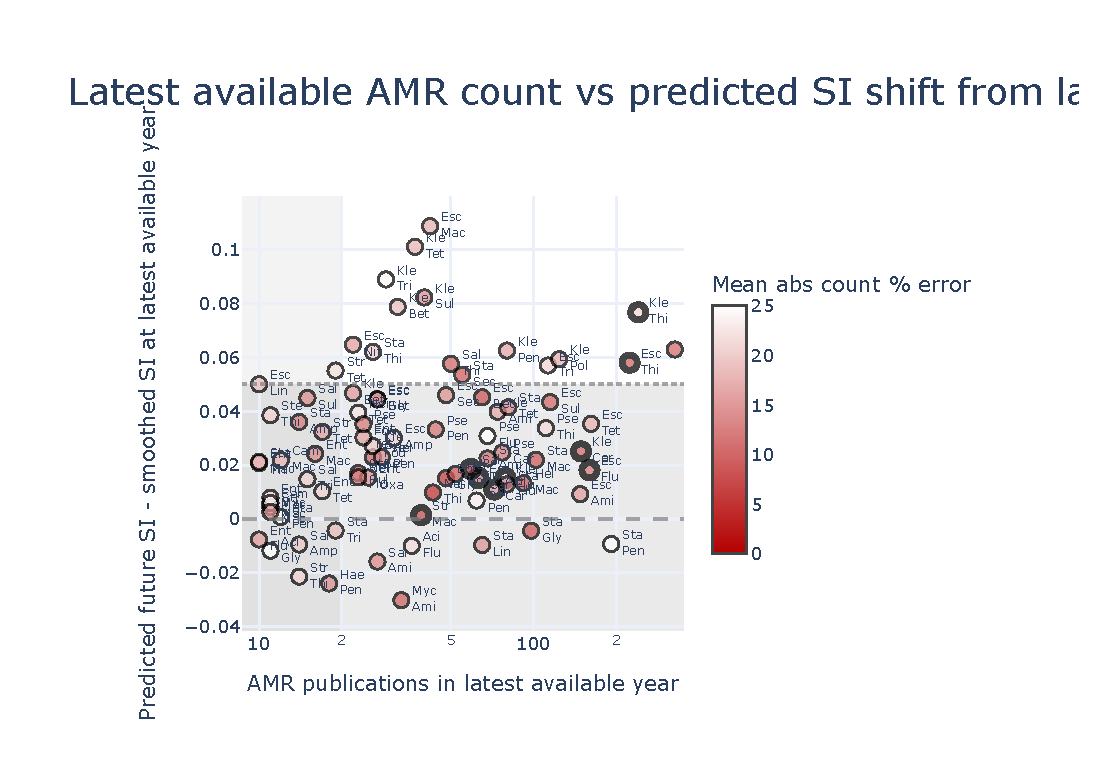
\includegraphics[width=0.9\textwidth]{../archive/legacy_notebooks/latest_observed_count_vs_future_si_shift.pdf}
\caption{Five-year SI-shift candidates after support and backtest filtering}
\label{fig:latest-count-vs-future-shift}
\end{figure}

Figure~\ref{fig:latest-count-vs-future-shift} makes the next-stage selection logic more explicit. It plots
the latest observed publication count for each eligible pair against the
predicted five-year increase in scientific interest, after filtering to
pairs that have enough observed publication support and low
holdout-period count prediction error. Pair-level Granger analysis is
therefore restricted to a filtered subset rather than applied across the
full sparse panel. The proposal uses the
forecasting baseline as a triage device: candidate pairs for the
leading-signal analysis are those that (i) have enough literature
support to define a usable yearly trajectory, (ii) can be forecast with
acceptable accuracy when the last five years are withheld, and (iii)
show a materially positive predicted SI shift. In other words, the
Granger stage is restricted to the part of the panel where both signal
density and baseline predictability are defensible.

\begin{table}[htbp]
\centering
\caption{Approximate supervised training examples from yearly SI trajectories}
\label{table-3-approximate-supervised-training-examples-from-yearly-si-trajectories}
\begin{tabular}{@{}lr@{}}
\toprule
Forecast setup & Approximate examples \\
\midrule
1-year-ahead future-SI examples & 31,948 \\
3-year-ahead future-SI examples & 23,920 \\
5-year-ahead future-SI examples & 19,301 \\
\bottomrule
\end{tabular}
\end{table}

These counts should be interpreted as pair-year training opportunities
derived from the screened yearly SI panel, not as independent biological
events. They provide an upper bound on the supervised examples available
before additional splitting constraints, rolling validation windows, or
feature-availability filters are applied.

\begin{figure}[htbp]
\centering
\includegraphics[width=0.88\textwidth]{../archive/legacy_assets/interesting_yearly_si_pngs_simplified_categories/Escherichia_coli__Penicillins.png}
\caption{Example of a dense yearly SI trajectory}
\label{fig:dense-si-trajectory}
\end{figure}

The archived simplified-category SI plot for \emph{Escherichia coli} and
Penicillins is a useful counterexample to the concern that all
trajectories are sparse. It also illustrates why coarser antibiotic
representations can be valuable: when related drugs are aggregated into
a therapeutic class, the resulting signal is often denser, smoother, and
more interpretable than many individual-drug trajectories. This is
exactly why the proposal treats antibiotic-class modeling as a credible
companion to individual-antibiotic prediction, especially for
short-horizon forecasting and robustness analysis.

\subsubsection{Scientific interest time-series
construction}\label{42-scientific-interest-time-series-construction}

For each antibiotic-pathogen pair, the project will compute yearly
publication counts representing research attention.

Additional bibliometric indicators may include:

\begin{itemize}
\tightlist
\item
  Normalized publication counts.
\item
  Citation-based measures.
\item
  Journal impact indicators.
\end{itemize}

The current codebase defines the core yearly SI target through a pooled
background-adjusted baseline. Specifically, yearly pair counts are
merged with yearly pathogen background counts and yearly antibiotic
background counts. A pooled ridge regression model is then fit on
log-transformed counts using:

\begin{itemize}
\tightlist
\item
  \(\log_{10}(1 + n_{\mathrm{pathogen},t}^{\mathrm{bg}})\)
\item
  \(\log_{10}(1 + n_{\mathrm{antibiotic},t}^{\mathrm{bg}})\)
\item
  pathogen indicator variables
\item
  antibiotic indicator variables
\end{itemize}

This yields an expected log pair count,
\( \widehat{\ell}_{\mathrm{pair},t}^{\mathrm{global}} \), and
scientific interest is
defined as:

\[
\mathrm{SI}_t
= \log_{10}(1 + n_{\mathrm{pair},t})
- \widehat{\ell}_{\mathrm{pair},t}^{\mathrm{global}}.
\]

These SI values form the baseline time series used for forecasting
future attention dynamics. This definition is important because it
measures pair-specific excess attention relative to general background
prominence, not just absolute publication volume. The same construction
can also be applied to broader antibiotic classes when a coarser and
denser representation is preferable to individual-drug modeling.

\subsubsection{Concept extraction from
abstracts}\label{43-concept-extraction-from-abstracts}

To capture higher-level AMR signals, the project will identify
conceptual indicators within scientific abstracts.

The first concept layer will focus on five concrete indicator types:

\begin{itemize}
\tightlist
\item
  documented treatment failure or reduced clinical efficacy for the
  focal antibiotic-pathogen pair
\item
  identification of a resistance mechanism, such as a resistance gene,
  enzyme, mutation, or efflux process
\item
  reports of epidemiological spread, outbreaks, or geographic expansion
  of resistant strains
\item
  surveillance or prevalence evidence indicating increasing resistance
  frequency in isolates or cohorts
\item
  diagnostic or susceptibility-testing signals indicating newly
  recognized resistance phenotypes
\end{itemize}

A language model will evaluate the presence of each indicator type in an
abstract and assign a graded score representing the strength of
association. Scores will be aggregated annually to produce
concept-specific time-series signals.

This approach allows the system to detect early changes in how
antibiotic-pathogen interactions are discussed in the literature.

The existing unified LLM filter also provides a foundation for this
stage because it already performs abstract-level, pair-specific judgment
rather than relying on raw co-occurrence. In practice, this means later
concept extraction can be applied to a cleaner corpus of pair-resolved
AMR-relevant abstracts, reducing contamination from papers that merely
mention the antibiotic and pathogen without asserting a relevant
resistance relationship.

The project is therefore not based on naive document-level co-mention
counts. Instead, it uses broad retrieval for recall and then applies
pair-specific LLM adjudication to decide whether a paper contributes
evidence to the focal antibiotic-pathogen trajectory.

\subsubsection{Semantic representation of literature
context}\label{44-semantic-representation-of-literature-context}

In addition to explicit conceptual signals, the project will model
latent semantic patterns in the literature.

Abstracts mentioning a given pathogen or antibiotic will be embedded
using biomedical language models. Embeddings will be averaged annually
to generate vector representations capturing the evolving discourse
surrounding each entity.

These semantic signals may capture subtle changes in scientific
narratives that precede increases in publication activity.

\subsubsection{Predictive modeling}\label{45-predictive-modeling}

The extracted signals will be integrated within a predictive modeling
framework that moves from simple baselines to more expressive sequence
models only when the data support that progression.

A preliminary baseline already fits a LOESS curve to yearly log counts
for each antibiotic-pathogen pair, uses damped linear tails for
extrapolation when forecasting beyond the observed range, and then
derives predicted SI by subtracting the interpolated expected log-count
baseline from the predicted log count. This provides a concrete
benchmark for future work.

The proposed extension is to move beyond this count-only forecasting
baseline in a staged way. Granger-causality analysis is first used to
identify signals that show consistent predictive temporal relationships
with future attention or SI. In this role, Granger analysis provides a
transparent and interpretable account of which signals appear to lead
the target and therefore offers a principled first view of the temporal
structure in the data. Those same signals can then be integrated into
progressively richer predictive models whose purpose is different: not
primarily interpretability, but stronger prediction through automatic
learning of when different combinations of signals are useful. The
first stage will examine linear regression and related additive models
that provide transparent baselines for multi-signal integration. The
next stage will evaluate convolutional sequence models to test whether
short-range temporal motifs across signals improve prediction. A
sequence transformer remains a candidate later-stage model for settings
where the available data are sufficiently rich and where validation
results show that a more expressive architecture materially improves
performance. Model selection is therefore empirical rather than
doctrinal: the final predictive architecture should be whichever level
of complexity is best supported by the data and by out-of-sample
predictive gain, even if the most powerful model is less transparent
than the earlier Granger-based analysis.

Conceptually, the model integrates:

\begin{itemize}
\tightlist
\item
  Historical scientific attention.
\item
  Conceptual AMR indicators.
\item
  Semantic context vectors.
\item
  Pathogen descriptors.
\item
  Antibiotic descriptors.
\end{itemize}

The system would predict future publication counts and future SI at time
horizons of one to five years, with the current LOESS-based SI
forecaster serving as the baseline comparator and the transformer
serving as a later-stage, more expressive model. For pairs with limited
support, the same short-horizon prediction task can also be defined at
the antibiotic-class level to improve density and robustness.

\subsubsection{Evaluation and
benchmarking}\label{46-evaluation-and-benchmarking}

The predictive framework will be evaluated using retrospective
validation.

Baseline models will include:

\begin{itemize}
\tightlist
\item
  Linear trend extrapolation.
\item
  Autoregressive time-series models.
\item
  Nonparametric smoothing approaches, including the existing LOESS-based
  forecaster.
\end{itemize}

Performance will be measured using predictive accuracy on both counts
and SI, along with the ability to detect emerging attention trajectories
earlier than baseline models. Because the codebase already computes
post-fit holdout errors for predicted SI, the evaluation framework can
be anchored in directly observed pair-level forecasting error rather
than only qualitative hotspot identification.

Crucially, the evaluation should test whether abstract-derived signals
improve prediction beyond publication momentum alone. That means the
central benchmark is not simply whether the proposed model forecasts
well in absolute terms, but whether it outperforms autoregressive and
trend-based baselines built only from historical pair counts or
historical SI. The main novelty claim of the project is therefore not
that SI is forecastable at all, but that there exist causal or leading
predictors in the literature that improve future-SI prediction beyond
past-SI-only models. Evaluation should prioritize short horizons of one
to five years, where the forecasting task is most credible, and can be
repeated at both the individual-antibiotic and antibiotic-class levels.

The evaluation design will therefore include an explicit ablation and
sensitivity framework rather than treating these comparisons as optional
side analyses. At minimum, the proposal commits to comparing:

\begin{itemize}
\tightlist
\item
  past-SI-only models versus multi-signal models
\item
  \texttt{yes}-only screening versus \texttt{yes} +
  \texttt{uncertain} screening
\item
  individual-antibiotic prediction versus antibiotic-class aggregation
\item
  linear models versus convolutional sequence models versus
  transformer-style models
\end{itemize}

These comparisons are central to the credibility of the design because
they test whether the proposed gains actually come from richer signals,
broader inclusion rules, coarser aggregation levels, or increased model
complexity. Without these ablations, it would be much harder to
interpret any performance improvement.

\subsubsection{Expected methodological
contribution}\label{expected-methodological-contribution}

The proposed framework combines four methodological elements that are
rarely integrated in AMR analysis:

\begin{enumerate}
\def\labelenumi{\arabic{enumi}.}
\tightlist
\item
  Pair-level LLM-based disambiguation of AMR evidence from broad
  literature retrieval.
\item
  Background-adjusted SI as a pair-specific bibliometric target.
\item
  Semantic and concept-level signals extracted from biomedical text.
\item
  A staged temporal modeling pipeline that moves from interpretable
  Granger-based signal prioritization to sequence-transformer
  forecasting.
\end{enumerate}

Together, these components provide a scalable approach to forecasting
emerging AMR research priorities and identifying antibiotic-pathogen
pairs likely to become significant in the near future.

\subsection{Granger-Causality
Analysis}\label{granger-causality-analysis}

A key question in the proposed framework is not only whether
literature-derived signals can predict future scientific attention
toward antibiotic-pathogen pairs, but also which signals are most
informative and how they influence one another over time. Understanding
these dependencies is important both for interpretability and for
validating whether the proposed signals capture meaningful early
indicators of emerging AMR concerns.

To address this question, the project will employ Granger causality
analysis, a statistical framework for identifying predictive
dependencies between time series.

\subsubsection{Conceptual overview}\label{51-conceptual-overview}

Granger causality provides a formal method for testing whether past
values of one time series improve the prediction of another time series
beyond what can be achieved using the past of the target variable alone.

Formally, a variable X is said to Granger-cause a variable Y if
including past observations of X significantly improves the prediction
of Y compared with a model that uses only past values of Y.

It is important to emphasize that Granger causality does not establish
true mechanistic causation. Instead, it identifies predictive temporal
dependencies, which are often useful indicators of underlying
relationships.

In the context of AMR literature analysis, this framework can be used to
determine whether certain signals extracted from the literature
systematically precede increases in scientific attention or increases in
background-adjusted scientific interest.

\subsubsection{Application to literature-derived
signals}\label{52-application-to-literature-derived-signals}

The project will construct several types of time-series signals for each
antibiotic-pathogen pair:

\begin{itemize}
\tightlist
\item
  Scientific attention signals, including yearly publication counts and
  the background-adjusted SI series already defined in the current
  codebase.
\item
  Conceptual signals extracted from abstracts, such as treatment
  failure, resistance mechanisms, and epidemiological spread.
\item
  Semantic context signals, including embedding-based representations of
  how pathogens or antibiotics are discussed in the literature.
\item
  Contextual descriptors related to pathogen characteristics or
  antibiotic properties.
\end{itemize}

Granger causality tests can be used to evaluate whether any of these
signals consistently precede increases in scientific attention or SI.

To make this stage reviewable, Granger analysis will not be applied to
all screened pairs. A pair will be eligible only if it satisfies a
three-part filter derived from the existing forecasting pipeline.
First, it must have enough publication support to define a meaningful
yearly series, operationalized as a minimum average yearly publication
count and at least 8 to 10 yearly observations after screening.
Second, the baseline SI/count forecaster must remain accurate under a
rolling five-year holdout test, so that the pair is not being analyzed
in a regime where even the target trajectory is unstable or dominated by
noise. Third, the pair must show a sufficiently large predicted future
increase in SI to justify treating it as an impending rise in
scientific salience rather than a negligible fluctuation. This means the
Granger question is narrowed from ``which auxiliary signals lead any
pair whatsoever?'' to ``which auxiliary signals lead the subset of
pairs with adequate support, demonstrable forecastability, and a large
expected rise in SI?''

This filtering also clarifies how the main statistical objections will
be handled. The target of the Granger analysis will be the yearly SI
series or its differenced form rather than raw sparse publication
counts, which reduces nonstationarity driven by long-run background
growth. Zero inflation is handled upstream by excluding extremely
low-support pairs and by requiring successful holdout prediction before
Granger testing is attempted. Multiple testing will be controlled using
false-discovery-rate correction across the family of pair-signal tests
within each analysis stage.

In practical terms, this involves comparing two models:

\begin{enumerate}
\def\labelenumi{\arabic{enumi}.}
\tightlist
\item
  A model predicting future scientific attention or future SI using only
  past values of the target signal.
\item
  A model predicting future scientific attention or future SI using past
  target values plus past values of another signal.
\end{enumerate}

If the second model significantly improves predictive performance, the
additional signal is said to Granger-cause the target signal. In the
context of this proposal, that comparison formalizes the central novelty
claim: whether signals other than past SI provide additional predictive
value for future SI.

\subsubsection{Resistance mechanism discovery preceding
research
attention}\label{53-example-1-resistance-mechanism-discovery-preceding-research-attention}

Consider a conceptual signal representing mentions of novel resistance
mechanisms in abstracts.

Let:

\begin{itemize}
\tightlist
\item
  \(A_t\) represent scientific attention or SI for a specific
  antibiotic-pathogen pair at year \(t\).
\item
  \(M_t\) represent the frequency of abstracts describing new
  resistance mechanisms.
\end{itemize}

If increases in \(M_t\) systematically occur before increases in
\(A_t\), the following regression model may reveal a
Granger-causal relationship:

\[
A_t = \alpha + \sum_i \beta_i A_{t-i} + \sum_i \gamma_i M_{t-i} + \varepsilon_t
\]

If the coefficients on the lagged \(M\) terms are statistically
significant, this suggests that discoveries of resistance mechanisms
tend to precede increases in scientific attention.

This would provide quantitative evidence that mechanistic discoveries
act as early signals of emerging AMR concerns.

\subsubsection{Epidemiological signals predicting
research
activity}\label{54-example-2-epidemiological-signals-predicting-research-activity}

Another conceptual signal may represent mentions of epidemiological
spread or outbreaks.

Let:

\begin{itemize}
\tightlist
\item
  \(E_t\) represent the frequency of abstracts describing
  epidemiological spread.
\end{itemize}

If epidemiological mentions precede increased publication activity or
increased SI, a Granger test may detect that lagged values of \(E\)
improve prediction of the attention signal.

Such a result would support the hypothesis that clinical or
public-health observations drive subsequent increases in research
activity.

\subsubsection{Semantic shifts in scientific
discourse}\label{55-example-3-semantic-shifts-in-scientific-discourse}

Semantic embeddings allow detection of changes in how pathogens or
antibiotics are discussed in the literature.

For instance, a semantic dimension might capture increasing emphasis on:

\begin{itemize}
\tightlist
\item
  Multidrug resistance.
\item
  Treatment failure.
\item
  Hospital-acquired infection.
\end{itemize}

Changes in these embedding components may precede increases in
publication volume or pair-level SI.

Granger analysis can test whether shifts in semantic context vectors
predict subsequent increases in attention signals.

This approach enables detection of latent narrative changes in the
literature before they manifest as large increases in publication
counts.

\subsubsection{Multi-variable Granger
analysis}\label{56-multi-variable-granger-analysis}

Beyond pairwise testing, the project will explore multivariate Granger
causality, where multiple signals are considered simultaneously.

Vector autoregressive (VAR) models provide a natural framework for such
analysis.

Using VAR models, it becomes possible to examine networks of predictive
dependencies among signals such as:

\begin{itemize}
\tightlist
\item
  Resistance mechanism discovery.
\item
  Epidemiological spread.
\item
  Diagnostic innovation.
\item
  Treatment failure.
\item
  Scientific attention.
\item
  Background-adjusted SI.
\end{itemize}

This analysis can reveal predictive pathways in the evolution of
scientific attention, helping to identify which signals consistently act
as early indicators.

\subsubsection{Relationship with the predictive
model}\label{57-relationship-with-the-predictive-model}

Granger causality analysis serves two complementary roles in the
proposed framework.

First, it provides interpretability by identifying which
literature-derived signals precede increases in scientific attention or
SI.

Second, it helps guide feature selection and model design by
highlighting which signals carry predictive information beyond past-SI
dynamics alone.

Signals identified as Granger-causal can be prioritized in the later
sequence-transformer stage of the predictive architecture described in
the methodology. In this way, Granger analysis acts as an
interpretability and feature-selection bridge between the current LOESS
benchmark and the more powerful transformer-based predictor.

\subsubsection{Expected insights}\label{58-expected-insights}

Applying Granger causality in this context can help answer questions
such as:

\begin{itemize}
\tightlist
\item
  Do reports of treatment failure precede increases in research
  attention?
\item
  Do discoveries of resistance genes predict future publication
  activity?
\item
  Do shifts in scientific discourse anticipate emerging AMR concerns?
\item
  Do some signals predict changes in background-adjusted SI more
  strongly than they predict raw publication volume?
\end{itemize}

If consistent predictive dependencies are identified, this would provide
stronger evidence that scientific literature contains measurable early
signals of emerging antimicrobial resistance issues.

Such findings would support the broader goal of the project: developing
a data-driven early-warning system based on the dynamics of scientific
attention.

\section*{References}

\begin{enumerate}
\item World Health Organization. \emph{Antimicrobial resistance: global report on surveillance}. WHO, 2014. \url{https://www.who.int/publications/i/item/9789241564748}
\item Pritchard, A. \emph{Statistical bibliography or bibliometrics?} Journal of Documentation, 1969. \url{https://doi.org/10.1108/eb026482}
\item Borromeo et al. \emph{Southeast-Asian landscape of antimicrobial resistance research}. \url{https://pubmed.ncbi.nlm.nih.gov/40983143/}
\item Sweileh et al. \emph{Bibliometric analysis of peer-reviewed literature on antimicrobial stewardship}. \url{https://pubmed.ncbi.nlm.nih.gov/33397377/}
\item Lin et al. \emph{Global insights into MRSA bacteremia: a bibliometric analysis and future outlook}. \url{https://pubmed.ncbi.nlm.nih.gov/39911705/}
\item \emph{Trends in antimicrobial resistance education research}. \url{https://pubmed.ncbi.nlm.nih.gov/40677968/}
\item Chen. \emph{CiteSpace II: Detecting and visualizing emerging trends and transient patterns in scientific literature}. \url{https://onlinelibrary.wiley.com/doi/10.1002/asi.20317}
\item Rotolo, Hicks, Martin. \emph{What Is an Emerging Technology?} \url{https://arxiv.org/abs/1503.00673}
\item Wang. \emph{A bibliometric model for identifying emerging research topics}. \url{https://asistdl.onlinelibrary.wiley.com/doi/10.1002/asi.23930}
\item Liang et al. \emph{Combining deep neural network and bibliometric indicator for emerging research topic prediction}. \url{https://www.sciencedirect.com/science/article/pii/S0306457321001072}
\item Min, Bu, Sun. \emph{Predicting scientific breakthroughs based on knowledge structure variations}. \url{https://www.sciencedirect.com/science/article/pii/S0040162520313287}
\item Ta\c{s}k{\i}n, Z. et al. \emph{Forecasting the future of library and information science and its sub-fields}. Scientometrics, 2021. \url{https://doi.org/10.1007/s11192-020-03800-2}
\item Porter et al. \emph{Emergence scoring to identify frontier R\&D topics and key players}. \url{https://www.sciencedirect.com/science/article/pii/S0040162517314804}
\item Xu et al. \emph{Multidimensional scientometric indicators for the detection of emerging research topics}. \url{https://www.sciencedirect.com/science/article/pii/S0040162520313160}
\item Huang et al. \emph{Tracking the dynamics of co-word networks for emerging topic identification}. \url{https://www.sciencedirect.com/science/article/pii/S0040162521003760}
\item Zhong et al. \emph{Bibliometric analysis of carbapenem-resistant Enterobacteriaceae research, 2010-2020}. \url{https://pubmed.ncbi.nlm.nih.gov/34237952/}
\item Maimaiti et al. \emph{Global trends and hotspots of phage therapy for bacterial infection}. \url{https://pubmed.ncbi.nlm.nih.gov/36699585/}
\item Lee J. et al. \emph{BioBERT: a pre-trained biomedical language representation model for biomedical text mining}. \url{https://doi.org/10.1093/bioinformatics/btz682}
\item Vaswani A. et al. \emph{Attention Is All You Need}. \url{https://arxiv.org/abs/1706.03762}
\item National Center for Biotechnology Information (NCBI). \emph{PubMed database}. \url{https://pubmed.ncbi.nlm.nih.gov}
\item Cleveland W.S. \emph{Robust locally weighted regression and smoothing scatterplots}. \url{https://doi.org/10.1080/01621459.1979.10481038}
\item Granger C.W.J. \emph{Investigating causal relations by econometric models and cross-spectral methods}. \url{https://doi.org/10.2307/1912791}
\item Sims C.A. \emph{Macroeconomics and reality}. \url{https://doi.org/10.2307/1912017}
\end{enumerate}


\appendix
\clearpage
\section{Proposal Review}\label{proposal-review}

\subsection{Summary judgment}\label{summary-judgment}

This is a strong proposal if it is judged as a scientometric prediction
project and a more vulnerable proposal if it is judged as a direct AMR
forecasting project. Its core idea is clear: model future
background-adjusted scientific interest for antibiotic-pathogen pairs
and test whether richer literature-derived signals improve that
prediction. That is a real and defensible research question.

The proposal is less convincing when it leans too close to claiming that
future scientific salience is already a proxy for future AMR burden. The
project may eventually support that broader interpretation, but the
proposal as written does not yet establish it.

\subsection{Major strengths}\label{major-strengths}

\subsubsection{1. The proposal has a real target, not a vague ML
objective}\label{the-proposal-has-a-real-target-not-a-vague-ml-objective}

Many proposals in this space collapse into a generic ambition to ``apply
AI to the literature.'' This one does not. It defines a target variable,
scientific interest, in a precise way and grounds it in a
background-adjusted residual rather than raw publication volume. That is
important because it turns the problem into a coherent prediction task
instead of a loosely defined bibliometric exercise.

\subsubsection{2. The data-construction workflow is
serious}\label{the-data-construction-workflow-is-serious}

The proposal is strongest where it treats measurement as part of the
scientific problem. The use of pair-specific LLM adjudication after
broad retrieval is a good example. It directly addresses the fact that
simple co-mention is not enough and that the quality of the pair-level
signal depends on a credible screening step.

This gives the project a more defensible foundation than a naive
document-counting pipeline would have had.

\subsubsection{3. The proposal is realistic about
sparsity}\label{the-proposal-is-realistic-about-sparsity}

The dataset section is one of the strongest parts of the document. It
shows counts, filtered trajectory lengths, and a practical fallback to
class-level aggregation. That matters because the proposal's credibility
depends heavily on whether it appears to understand its own data regime.

It does.

\subsubsection{4. The signal design is more concrete than in most
literature-mining
proposals}\label{the-signal-design-is-more-concrete-than-in-most-literature-mining-proposals}

The concept-extraction stage now has identifiable signal families rather
than generic promises about latent NLP features. Treatment failure,
resistance mechanisms, epidemiological spread, surveillance signals, and
diagnostic signals are concrete enough that a reviewer can understand
what is being measured and why those variables might matter.

The same is true of the semantic-embedding section, which now gives a
clear reason for embeddings beyond feature inflation: they are intended
to support similarity-based generalization across related pathogens,
related antibiotics, and sparse pairs.

\subsubsection{5. The modeling section is much more disciplined than a
transformer-first
pitch}\label{the-modeling-section-is-much-more-disciplined-than-a-transformer-first-pitch}

The proposal's decision to move from simpler models to more expressive
ones is good. Starting from linear or additive models, then considering
convolutional sequence models, and only using transformer-style models
if they are actually supported by the data is the right posture.

This also improves the proposal's scientific tone, because it frames
model choice as something to be earned through evidence rather than
announced in advance.

\subsection{Main weaknesses}\label{main-weaknesses}

\subsubsection{1. The project's external meaning remains the largest
unresolved
issue}\label{the-projects-external-meaning-remains-the-largest-unresolved-issue}

The proposal is clear that the immediate target is future scientific
interest. That is good. But the wider motivation still depends on the
idea that forecasting future scientific interest says something useful
about future AMR concern in the world, not just in the literature.

That bridge is plausible, but not yet demonstrated. Without an external
benchmark of some kind, the proposal remains vulnerable to a simple
criticism: that it forecasts the future attention of researchers rather
than the future trajectory of resistance itself.

This is not a fatal flaw, but it is the central one.

\subsubsection{2. The Granger stage is still the shakiest part of the
methodology}\label{the-granger-stage-is-still-the-shakiest-part-of-the-methodology}

The proposal is persuasive when it uses Granger analysis as an
interpretability tool and signal-prioritization device. It is less
persuasive when it treats Granger analysis as if it were straightforward
to defend on short, filtered, noisy yearly series.

A reviewer is likely to ask:

\begin{itemize}
\tightlist
\item
  how many time points are truly required
\item
  what lag structure is searched
\item
  whether the analysis is run on SI levels or differences
\item
  how zero-heavy or unstable trajectories are excluded
\item
  how multiple testing is controlled
\end{itemize}

The proposal points in the right direction, but it still needs more
hard-edged operational detail here than it currently provides.

\subsubsection{3. The distinction between individual-drug and
class-level analyses needs sharper scientific
framing}\label{the-distinction-between-individual-drug-and-class-level-analyses-needs-sharper-scientific-framing}

The class-level fallback is practical and probably necessary, but it
changes the meaning of the task. Predicting future salience for a single
antibiotic-pathogen pair is not the same scientific question as
predicting future salience for an antibiotic class against a pathogen.

The proposal knows that class-level aggregation helps with sparsity. It
does not yet say clearly enough what is gained scientifically and what
is lost when this switch happens.

\subsubsection{4. The screening-rule sensitivity problem remains
important}\label{the-screening-rule-sensitivity-problem-remains-important}

Including \texttt{uncertain} rows may be reasonable, but it is not a
neutral choice. It changes the evidence base from which SI is
constructed. The proposal is right to include a sensitivity plan, but
this issue is important enough that it should be framed as central to
the validity of the measurement model, not merely as a robustness check.

\subsubsection{5. The proposal still relies on a few interpretive
leaps}\label{the-proposal-still-relies-on-a-few-interpretive-leaps}

The strongest sections are concrete and operational. The weaker sections
move too quickly from:

\begin{itemize}
\tightlist
\item
  literature-derived signal
\item
  to rising scientific salience
\item
  to future AMR concern
\end{itemize}

Those links may all be reasonable, but they are not equivalent, and the
proposal is best when it keeps those distinctions explicit.

\subsection{What would most improve the
proposal}\label{what-would-most-improve-the-proposal}

\subsubsection{1. Add one external validation
target}\label{add-one-external-validation-target}

This would improve the proposal more than any increase in model
complexity. Even a modest external anchor would help establish why
future-SI prediction matters.

Examples could include:

\begin{itemize}
\tightlist
\item
  surveillance trend data
\item
  external AMR priority lists
\item
  curated historical resistance escalations
\end{itemize}

\subsubsection{2. Make eligibility rules explicit and
numerical}\label{make-eligibility-rules-explicit-and-numerical}

The proposal should state concrete thresholds for:

\begin{itemize}
\tightlist
\item
  minimum yearly observations
\item
  minimum publication support
\item
  acceptable holdout error
\item
  Granger eligibility
\item
  when to switch from individual drugs to class-level models
\end{itemize}

That would turn the proposal from a plausible design into a much more
reviewable one.

\subsubsection{3. Treat ablation as a central result, not a
supplementary
check}\label{treat-ablation-as-a-central-result-not-a-supplementary-check}

The proposal is right to commit to comparisons between:

\begin{itemize}
\tightlist
\item
  past-SI-only and multi-signal models
\item
  \texttt{yes}-only and \texttt{yes\ +\ uncertain}
\item
  individual-drug and class-level analyses
\item
  linear, convolutional, and transformer-style models
\end{itemize}

Those comparisons should be framed as core outputs of the project
because they determine whether the richer modeling actually adds value
or merely adds flexibility.

\subsection{Final view}\label{final-view}

This proposal has genuine substance. It has a coherent target, a
credible measurement workflow, a realistic view of sparsity, and a more
disciplined modeling strategy than many proposals in this area.

Its main challenge is not that it lacks technical ideas. Its main
challenge is that the broader meaning of success still depends on an
external connection that the current design only argues for, rather than
directly demonstrates.

If the project adds one external validation layer and tightens the
eligibility rules for the more fragile stages, it becomes a much more
compelling proposal.


\end{document}
